\section{Introduction}

A variety of applications need a lower dimensional, concise and faithful representation of the original parent geometry. A skeleton is such an entity which represents the shape of its parent object. It being simpler than the parent object, applications like pattern recognition, approximation, similarity estimation, collision detection, animation, matching and deformation can be performed efficiently on it than on the parent object. 

Approaches such as Medial Axis Transform (MAT),  Chordal Axis Transform (CAT), Thinning etc. are used to compute skeletons. Table \ref{Medials} briefly summarizes some of these along with their strengths and weaknesses. In this paper, terms like 'Skeleton', 'Midcurve' and 'Medial' are used synonymously.

%\vspace{-2em}
\begin{table}[!h]
\caption{Current medial computation methods (see online version for colours)}
\begin{tabular}[htb]{@{}  p{0.15\linewidth} | p{0.2\linewidth} | p{0.3\linewidth} | p{0.2\linewidth} @{}} \toprule
%\begin{tabular}[h]{@{} l l l l @{}} \toprule
{\bf Method }  & {\bf Figure} & {\bf Description} & {\bf Problems}\\
\midrule
%------------------------------------------------------------------------------------------------------------------------------------
Medial Axis Transform \citep{Ramanathan2004}  &
\raisebox{-.9\height}{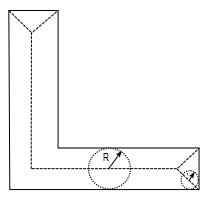
\includegraphics[width=\linewidth]{..//Common/images/MAT.png} }&
The loci of centers of the maximal circle in 2D, the ball in 3D. The radius function denotes the thickness. 
 &
Unwanted branches at the corners. \added[]{Sensitive to perturbations}.\\

\midrule
%------------------------------------------------------------------------------------------------------------------------------------
Chordal Axis Transform \citep{Quadros2008} &
\raisebox{-.9\height}{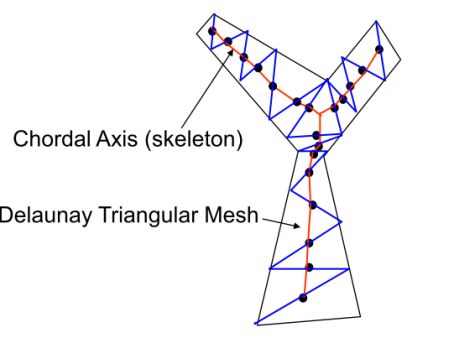
\includegraphics[width=\linewidth]{..//Common/images/CAT.png}}&
Triangulates the profile. Joins midpoints of the chords to form a medial.  &
Gaps at end. Expensive triangulation. \\
\midrule

%------------------------------------------------------------------------------------------------------------------------------------
Straight Skeleton \citep{Haunert2004}  &
\raisebox{-.9\height}{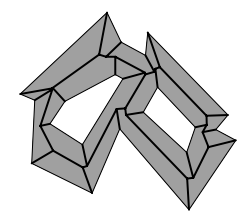
\includegraphics[width=\linewidth]{..//Common/images/Straight.png}} &
\replaced[]{Starts thinning from the boundary towards inside; stops at the meeting points}. &
Bisectors are not equidistant.\\

\bottomrule
\end{tabular}
\label{Medials}
\end{table}
%\vspace{-1em}
This paper focuses on 2D planar sketch profiles with an assumption that curved shapes can be converted to polygonal shape by faceting. Divide-and-Conquer has been used where Decomposition partitions the given shape into sub-shapes and skeletonization creates the midcurves in simpler sub-polygons.  At the end, individual midcurves are extended and joined to form a continuous set of curves mimicking the parent shape.

